\subsubsection{Exercise}
\paragraph{Minimum phase model}

Figure \ref{singm} shows the maximum and minimum singular value of $S$ and $T$ as a function of the frequency. 
In this minimum-phase case, no restricting criteria was formulated regarding to $S$ and $T$.

\begin{figure}[h!t]
    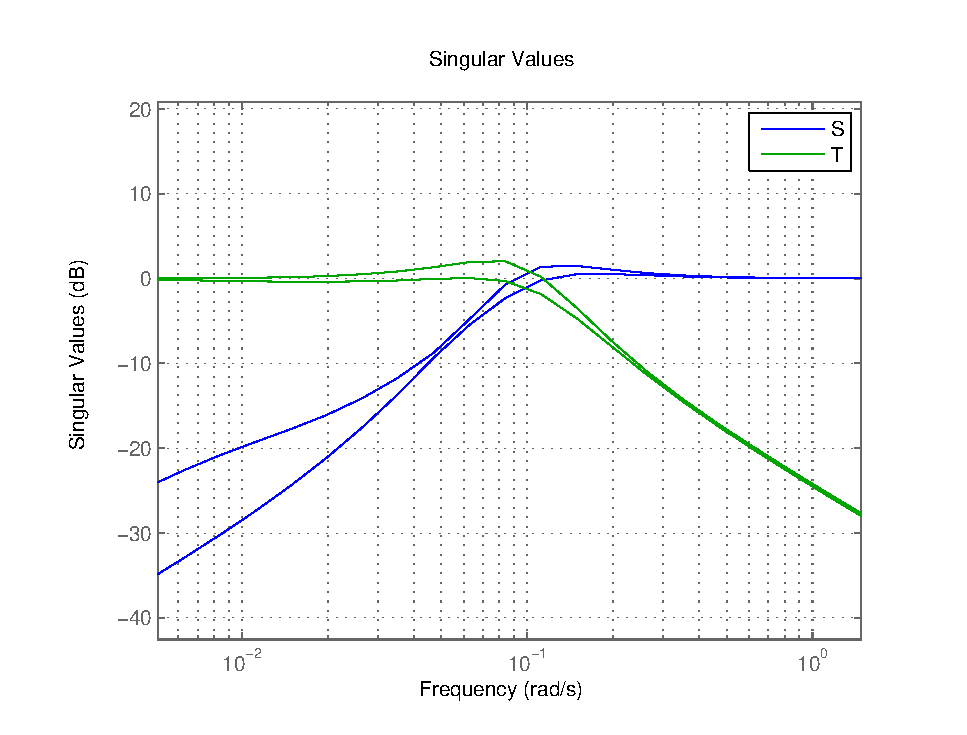
\includegraphics[width=\columnwidth]{fig/ST322m.eps}
    \caption{Singular values of $S$ and $T$ for the minimum phase system}
    \label{singm}
\end{figure}

\paragraph{Non-minimum phase model}


Figure \ref{singnm} shows the maximum and minimum singular value of $S$ and $T$ as a function of the frequency. 
In this non-minimum-phase case, since there is a RHP zero in the transfer matrix we had the following criteria regarding the bandwith limitation : $\omega_{BS} \leq 0.029$. This criteria is fulfilled.


\begin{figure}[h!t]
    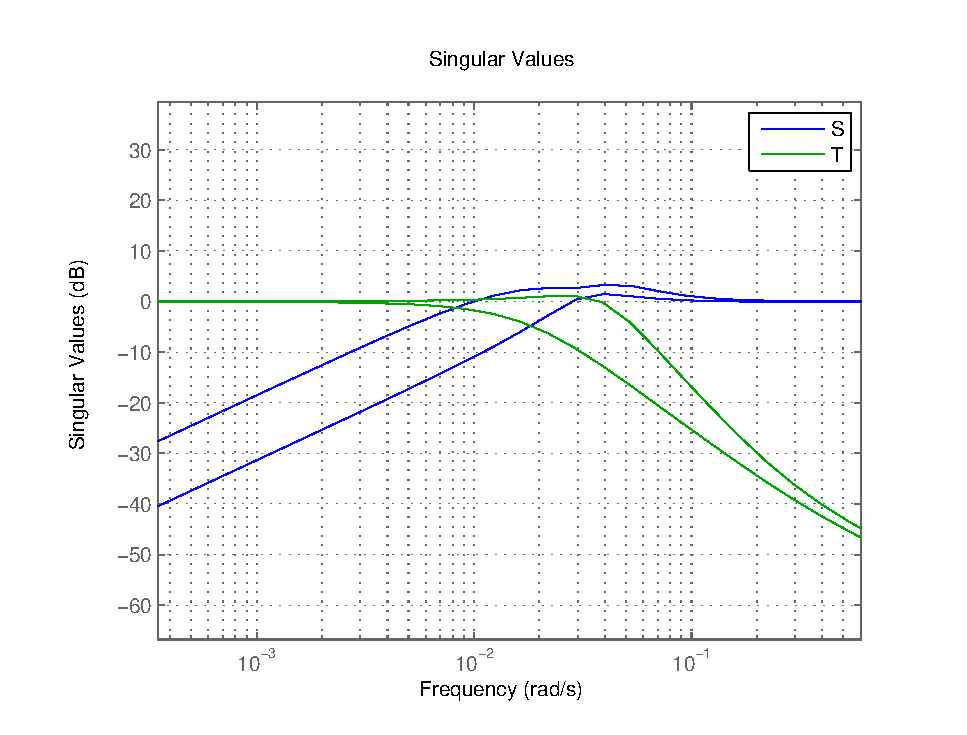
\includegraphics[width=\columnwidth]{fig/ST322nm.eps}
    \caption{Singular values of $S$ and $T$ for the non-minimum phase system}
    \label{singnm}
\end{figure}

